\documentclass[lang=cn,10pt]{elegantbook}
\usepackage{graphicx}
\usepackage{float}
\usepackage{gensymb}
\usepackage{txfonts}
\setmainfont{TeX Gyre Termes}
\title{课堂笔记}



\author{ Huang}



\setcounter{tocdepth}{3}


\cover{cover.jpg}

% 本文档命令
\usepackage{array}
\newcommand{\ccr}[1]{\makecell{{\color{#1}\rule{1cm}{1cm}}}}

% 修改标题页的橙色带
% \definecolor{customcolor}{RGB}{32,178,170}
% \colorlet{coverlinecolor}{customcolor}

\begin{document}
	
	\maketitle
	\frontmatter
	
	\tableofcontents
	
	\mainmatter
\chapter{多元函数的极限和连续}
\section{2023/8/31}
\begin{definition}
	$\text{设}F\subset \mathbb{R} ^n\text{,若}F^c\text{为开集,则称}F\text{为闭集}$
\end{definition}
\begin{theorem}
	在$\mathbb{R} ^n$中
	
	$1.\mathbb{R} ^n,\oslash$均为闭集(很特殊的一点,这两个同时为开集和闭集)
	
	$2.\text{若}{F_{\alpha}}$为$\mathbb{R} ^n$中的一个闭集族,其中指标$\alpha$来自一个指标集合$I$,则$\bigcap_{\alpha \in I}{F_{\alpha}}$也是闭集
	
	$3.$设$F_{1},F_{2},\cdots,F_{m}$为有限个闭集,则它们的并集$\bigcup_{i=1}^m{F_i}$也是闭集
\end{theorem}
令$\check{B}\left( a,r \right) =B\left( a,r \right) \backslash\{a\}\text{为以}a\text{为心,半径为}r\text{的空心球}$
\begin{definition}
	$\text{设}E\subset \mathbb{R} ^n$,若点$a\in \mathbb{R} ^n$满足:对任意$r>0$,在空心
	球 $\check{B}\left( a,r \right)$总含有$ E$ 中的点,则称 $a$ 为 $E$ 的聚点
\end{definition}
\begin{remark}
	聚点可以属于$ E $也可以不属于 $E$。若 $E $中的点不是
	聚点,则称其为孤立点。
\end{remark}
\begin{definition}
	$E\subset \mathbb{R} ^n$的凝聚点的全体称为 $E$ 的导集,记作
	$E′$,记$\bar{E}=E\cup E'$ ,称其为 $E$ 的闭包
\end{definition}
\begin{theorem}
	$E $为闭集的充要条件是 $E'\subset  E$,即$\bar{E}=E$
\end{theorem}
\begin{proof}
	
	$\Longrightarrow $我们要证明的是包含关系,于是先把$E'$中的元素设出来,不妨假设$x\in E'$,只需要证明$x\text{同时也}\in E$即可,但直接证明不是很好证明,考虑反证法,即$x\notin E\Rrightarrow x\in E^c$
	
	点在集合中,直接默写定义
	\begin{equation*}
		\exists r>0,\text{使得}  B(x,r)\subset E^c
	\end{equation*}
	
	于是乎,有
	\begin{equation}
		\hat{B}\left( x,r \right) \cap E=\oslash 
	\end{equation}
	
	根据聚点的定义,我们是对任意的$r>0$的去心球均有交集,但我们推出了如$(1.1)$的结论,表明其不为$E$的聚点,故
	\begin{equation*}
		x\in E'
	\end{equation*}
	与先前假设$x\in  E'$ 矛盾,于是假设错误
	
	$\Longleftarrow$现在我们要证明$E$为闭集通常像这类的证明,我们要将其转化为该集合的补集进行证明。故我们只需证明$E^{c}$为开集即可,但事实上,直接进行证明有些难度,我们采取反证法
	
	假设$E^{c}$非开,按定义直接写(把开集的定义反着来)
	\begin{equation*}
		\exists x \in E^{c},\forall r >0,B(x,r)\cap E\ne\oslash (\text{这里的结论是}B(x,r)\subset E^{c}\text{的反例,不属于这个集合,等价于和这个集合的补集有交集})
	\end{equation*}
	
	$x$显然不在$E$中,则$x$为$E$的一个聚点,于是有
	\begin{equation*}		
		x\in E' \subset E
	\end{equation*}
	与$x \in E^{c}$矛盾,假设错误
\end{proof}
\begin{corollary}
	$E $是闭集的充要条件是$ E $中的任何收敛点列的极限必
	在 $E$ 中
\end{corollary}
\begin{proof}
	$\Longrightarrow$设$\left\{ a_n \right\} \subset E$ 且$\underset{n\rightarrow \infty}{\lim}a_n=x$,直接证明不好证明,我们采取反证法,假设$x\in E^{c}$,又因为$E^{c}$为开集,按定义
	\begin{equation*}
		\exists r>0,B(x,r)\subset E^{c}
	\end{equation*}
	
	又因为$a_{n}$收敛于$x$,于是存在无穷多个$a_{n}$在$x$附近的一个开球$B(x,r)$中,故$x$为$E$的一个聚点于是有
	\begin{equation*}		
		x\in E' \subset E
	\end{equation*}
	
	与$x \in E^{c}$矛盾,假设错误
	
	$\Longleftarrow$现在我们要证明$E$为闭集通常像这类的证明,我们要将其转化为该集合的补集进行证明。故我们只需证明$E^{c}$为开集即可,但事实上,直接进行证明有些难度,我们采取反证法
	
	假设$E^{c}$非开,按定义直接写(把开集的定义反着来)
	\begin{equation*}
	\exists x \in E^{c},\forall r >0,B(x,r)\cap E\ne\oslash (\text{这里的结论是}B(x,r)\subset E^{c}\text{的反例,不属于这个集合,等价于和这个集合的补集有交集})
	\end{equation*}
	
	我们取$\left\{ a_n \right\} \subset B(x,r)\cap E\ne\oslash$使得$\underset{n\rightarrow \infty}{\lim}a_n=x$,(由收敛数列的稠密性,这是可以做到的)由题条件可知$x\in E$,矛盾

\end{proof}
\begin{corollary}
	完备度量空间的闭子集是完备集。
\end{corollary}
\begin{proof}
	只需要证明取出来的闭子集仍然是柯西列即可。
	
	$\forall \left\{ x_n \right\} \subset E$且$\left\{ a_n \right\}$在$E $中为柯西列,我们有
	\begin{equation*}
	\forall \varepsilon>0,\exists  N,\text{当}m,n>N\Rightarrow
	 \left\| x_n-x_m \right\| <\varepsilon 
	\end{equation*}
	
	于是完备
\end{proof}
\begin{theorem}
	$E $的导集 $E'$ 和闭包 $\bar E$ 均为闭集
\end{theorem}
\begin{proof}

	导集$E'$:
	
	由推论(1.1)我们只需要证明导集$E'$中的每个收敛点列都收敛到$E'$即可,设$\forall \text{收敛点列}\left\{ x_n \right\} \subset E'$且$\underset{n\rightarrow \infty}{\lim}x_n=x$,只需要证明$x\in E'$即可(即$x$为$E$的一个聚点)
	
	取$x_{1} \in E'$,存在$E$中的点列$\left\{ m_{k}^{1}} \right\}\rightarrow x_{1}$
	
	取$x_{2} \in E'$,存在$E$中的点列$\left\{ m_{k}^{2}} \right\}\rightarrow x_{2}$
	
	$\cdots$
	
	取$x_{k} \in E'$,存在$E$中的点列$\left\{ m_{k}^{k}} \right\}\rightarrow x_{k}$
	
	以此类推
	
	对于上述点列,我们采取以下取法:第一组点列取第一个点,第二组取第二个点,$\cdots$,第$k$组取第$k$个点,用这些点组成一个数列,现在我们要证明该数列收敛到$x$
	
	对于$\left\{ x_k \right\}$,我们有
	\begin{equation*}
	\forall \varepsilon>0 ,\exists N_{1},k>N_{1}\Rightarrow \left\| x_k-x \right\| <\varepsilon
	\end{equation*}
	
	因为$\left\{ m_{k}^{k}} \right\}\rightarrow x_{k}$,对于上述的$\varepsilon$,$\exists N_{2}$,$k>N_{2}$$\Rightarrow$$\left\| m_{k}^{k}-x_{k} \right\|<\varepsilon$
	
	取$N=\max \left\{ N_1,N_2 \right\} $,当$k>N$时,有
	\begin{equation*}
		\left\| m_{k}^{k}-x \right\| =\left\| m_{k}^{k}-x_k+x_k-x \right\| <\left\| m_{k}^{k}-x_k \right\| +\left\| x_k-x \right\| <2\varepsilon 
	\end{equation*}
	
	则$\underset{n\rightarrow \infty}{\lim}m_{k}^{k}=x$,我们找到了一组点列趋近于$x$,于是$x\in E'$,又因为该组点列是通过$\left\{ x_n \right\} \subset E'$所取得的,所以$E'$中的每个收敛点列都收敛到$E'$,得证
	
	闭包$\bar E$(本题也可以用上面的做法,但为了答案的多样性,采取另一种做法) :
	
	证明$\bar E$为闭,只需证明补集为开。令$x\in$ $\bar E^{c}$,则$x$不为$E$的聚点
	
	则存在$r_{1}>0$,使得$\check{B}(x,r_{1})\cap E=\oslash$
	
	取$x'\in \check{B}(x,r_{1})$,则存在$r_{2}$使得$ \check{B}(x',r_{2})\subset \check{B}(x,r_{1})$
	
	则$\check{B}(x',r_{2})$中的所有点都不是$E$的聚点,则$\check{B}(x,r_{2})\cap E=\oslash$
	
	于是$\forall x\in\bar E^{c}$,都存在一个领域包含于$\bar E^{c}$,于是$\bar E^{c}$为开集,故$\bar E$为闭集
\end{proof}
\section{2023/9/4}
\begin{theorem}
$	E\degree$是含于 $E$ 内的最大开集, $\bar E$是包含 $E $的最小闭
	集。
\end{theorem}
\begin{proof}
	
	若为最大开集,只需要证明任意的开集都是其子集即可。
	
	$\forall x \in E$,则存在$r_{1}>0$,使得$B(x,r_{1})\subset E$
	
	显然存在$m$和$r_{2}>0$,使得$B(m,r_{2})\subset B(x,r_{1})\subset E$
	
	由于$x$任意性,于是有$B(m,r_{2}) \subset E \degree$,得证
	
	要证是最小闭集,只需要证明任意的包含$E$的闭集都包含$\bar{E}$即可
	
	任取闭集$F$使得$E\subset F$,下证$\forall x \in \bar{E},x\in F  $
	
	由于$\bar{E}=E\cup E'$,下面分情况讨论
	
	1.$x\in E$,显然成立
	
	2.$x \in E'$,则$\forall r_{1}>0$,使得$\check{B}(x,r_{1})\cap E\ne\oslash$
	
    又$E\subset F$,则$\check{B}(x,r_{1})\cap F\ne\oslash$
    
    则$x\in \bar{F}$,又$F$为闭,则$\bar{F}=F$
    
    综上,$\forall x \in \bar{E},x\in F  $
\end{proof}
\begin{definition}
	设$E\subset \mathbb{R} ^n$,$	(E^{c})\degree $称为$E$的外点,$E$ 的外点的全体称
	为 $E$ 的外部;既不是 $E$ 的内点,也不是 $E$ 的外点的点称为 $E$ 的
	边界点,$E$ 的边界点的全体称为 $E$ 的边界,记为$\partial E$。
\end{definition}
\begin{remark}
	$a$ 为 $E$ 的外点,则存在一个球 $B(a, r)$ 使得其中完全
	不含有 $E$ 中的点;$b$ 是 $E$ 的边界点当且仅当对任何 $r > 0$,球
	$B(b, r)$ 均既含有 $E$ 中的点,也含有$ E^{c}$
	的点。
\end{remark}
\begin{example}
	求以下诸点集的内点、外点和边界点:
	
	1.$E=\mathbb{R} ^n$
	
	2.$E=\left\{ a \right\} \text{为单点集}$
	
	3. $E$ 为$\mathbb{R} ^2 $ 中的一条直线
	
	4.$E = B(a, r)$
\end{example}
\begin{solution}
	
	1.内点:$\mathbb{R} ^n$外点:$\oslash$边界点:$\oslash$
	
	2.内点:$\oslash$外点:$\mathbb{R} ^n/\left\{ a \right\} $边界点:$\left\{ a \right\}$
	
	3.内点:$\oslash$外点:$\mathbb{R} ^n/\left\{ \text{那条直线} \right\} $边界点:\left\{ \text{那条直线} \right\}
	
	4.内点:$E$ 外点:空间中挖去$E$和其边界点 边界点:球的边缘
\end{solution}
\begin{definition}
	设$E\subset \mathbb{R} ^n$,定义$E$的直径为
	\begin{equation*}
		\mathrm{diam}\left( E \right) =\mathrm{sup}\left\{ \left\| x-y \right\| :x,y\in E \right\} 
	\end{equation*}
\end{definition}
\begin{theorem}[$Cantor $闭集套定理]
	$\text{设}\left\{ F_i \right\} \left( F_i\ne \oslash ,i=1,2,\cdots ,n \right) \text{是一个闭集列},\text{且满足}$:
	
	1.$F_1\supset F_2\supset \cdots \supset F_n$
	
	2.$\underset{i\rightarrow +\infty}{\lim}\mathrm{diam}\left( F_i \right) =0$
	
	则存在唯一的点 $a $属于所有的 $F_{n}$
\end{theorem}
\begin{proof}
	
	先证明存在性,构造$\left\{ x_n \right\} 
	$,取法如下:
	
	取$x_{1} \in F_{1}$
	
	取$x_{2} \in F_{2}$
	
	$\cdots$
	
	取$x_{n} \in F_{n}$
	
	则$\forall \varepsilon >0 ,\exists N,i,j$,当$j>i>n>N$时,有
	\begin{equation*}
		\left\| x_i-x_j \right\| \le \mathrm{diam}\left( F_i \right) <\varepsilon 
	\end{equation*}
	
	由$Cauchy$收敛准则,极限存在
	
	再证明唯一性
	
	设$a,a'$均为$F_{i}$的极限,
	则
	\begin{equation*}
		\left\| a-a' \right\| \le \mathrm{diam}\left( F_i \right) \rightarrow 0
	\end{equation*}
	唯一性成立
\end{proof}
\section{2023/9/7}
\begin{definition}
	设$E\subset \mathbb{R} ^n$,如果 $E$ 中的任一点列都有一子列收敛于
	$E$ 中的一点,则称 $E$ 是 $\mathbb{R} ^n$中的列紧集(列紧集中的每个点都是聚点)
\end{definition}
\begin{theorem}[$Bolzano-Weierstrass $致密性定理]
$\mathbb{R} ^n$中的集合 $E$
	是列紧集的充要条件是 $E$ 为有界闭集
\end{theorem}
\begin{proof}
	
	$\Rightarrow$
	
	先证明有界($ps.$其实列紧性和紧致性是等价的)、
	
	正面做不好做,我们反证法
	
	假设其发散
	
	\begin{equation*}
		\forall M>0,\exists x\in E,\text{使得}\left\| x \right\| >M
	\end{equation*}
	
	接下来的手法需要积累
	
	取$M=1$,$\exists x_{1}\in E,\text{使得}\left\| x \right\| >M$
	
	取$M=\max \left\{ 2,\left\| x_1 \right\| +1 \right\} $,$\exists x_{2}\in E,\text{使得}\left\| x_{2} \right\| >M$
	
	$\cdots$
	
	取$M=\max \left\{ k,\left\| x_{k-1} \right\| +1 \right\} $,$\exists x_{k}\in E,\text{使得}\left\| x_{k} \right\| >M$
	
	这样取,构成了一个集合$\left\{ x_n \right\} 
	$
	
	由于$\left\{ x_n \right\} 
	 \subset E$是列紧集,故可选取子列使其收敛,不妨选取
	 $\left\{ x_{n_{k}} \right\} 
	 \subset\left\{ x_n \right\} 
	 \subset E$,其中$\left\{ x_{n_{k}} \right\} $收敛
	 
	 但事实上,$\exists N,n_{k_{1}}> n_{k_{2}}>N$
	 \begin{equation*}
	 	\left\| x_{n_{k_1}}-x_{n_{k_2}} \right\| >n_{k_1}-n_{k_2}
	 \end{equation*}
	 
	 此时发散,与子列收敛矛盾
	 
	再证明其为闭集
	
	只需证明$E$中所有收敛数列的极限都收敛到$E$中即可
	
	$\text{取}\left\{ x_n \right\} \subset E,\text{并且}\underset{n\rightarrow \infty}{\lim}x_n=x$
	
	对于$\left\{ x_n \right\}$,我们有
	\begin{equation*}
		\forall \varepsilon>0 ,\exists N_{1},n>N_{1}\Rightarrow \left\| x_n-x \right\| <\varepsilon
	\end{equation*}
	
	下证$x\in E$
	
	由于$E$是列紧集,则
	\begin{equation*}
		\exists \left\{ x_{n_{k}} \right\}\subset\left\{ x_n \right\},\text{使得}\underset{n\rightarrow \infty}{\lim}x_{_{n_{k}}}=x_{0}\in E
	\end{equation*}
	
	即
	
	\begin{equation*}
		\forall \varepsilon>0 ,\exists N_{2},n>N_{2}\Rightarrow \left\| x_{n_{k}}-x_{0} \right\| <\varepsilon
	\end{equation*}
	
	由于$x_{n_{k}}$为$x_{n}$子列,且$x_{n}$收敛
	,则有
	
	\begin{equation*}
		\forall \varepsilon>0 ,\exists N_{3},n>N_{3}\Rightarrow \left\| x_{n_{k}}-x_{n} \right\| <\varepsilon
	\end{equation*}
	
	取$N=\max \left\{ N_1,N_2,N_3 \right\} $
	\begin{equation*}
		\forall \varepsilon >0,n>N,\text{有}\left\| x-x_0 \right\| =\left\| x-x_n+x_n-x_{n_k}+x_{n_k}-x_0 \right\| <3\varepsilon 
	\end{equation*}
	则$x\in E$
	
	$\Leftarrow$
	
	由于$E$为有界闭集,则
	\begin{equation*}
		\forall x\in E,\exists \left\{ x_{n_k} \right\} \subset \left\{ x_n \right\} \subset E,\text{使得}\underset{n\rightarrow \infty}{\lim}x_{n_k}=x\in E
	\end{equation*}
	
	由此,$E$是列紧集
\end{proof}
\begin{definition}
	$\text{设}E\subset \mathbb{R} ^n\text{,}\mathcal{G} =\left\{ G_{\alpha} \right\} \text{为}\mathbb{R} ^n\text{中的一个开集族,如果}$
	\begin{equation*}
		E\subset\bigcup_{\alpha}{G_{\alpha}}
	\end{equation*}
	则称开集族 }$\mathcal{G}$覆盖了 $E$,或者称 }$\mathcal{G}$ 是 $E$ 的一个开覆盖
\end{definition}
\begin{definition}
	$\text{设}E\subset \mathbb{R} ^n$,若能从 $E$ 的任一个开覆盖中选出有限个
	开集,它们仍能组成 $E$ 的开覆盖,那么就称 $E$ 为一个紧致集
\end{definition}
\begin{theorem}[$Heine-Borel$ 有限覆盖定理]
	$ \mathbb{R} ^n$中的集合 $E$ 是紧致
	集的充要条件是 $E$ 为有界闭集
\end{theorem}
\begin{proof}
	
	$\Rightarrow$
	
	先证明有界
	
	由题,我们可以构造以下开覆盖
	\begin{equation*}
		\bigcup_{i=1}^{+\infty}{B\left( 0,i \right)}
	\end{equation*}
	
	显然有
	\begin{equation*}
		E\subset\mathbb{R} ^n \subset	\bigcup_{i=1}^{+\infty}{B\left( 0,i \right)}
	\end{equation*}
	
	由有限覆盖定理,$\exists m>0$使得
	\begin{equation*}
		E\subset	\bigcup_{i=1}^{m}{B\left( 0,i \right)}
	\end{equation*}
	
	显然有
	\begin{equation*}
		B(0,i)\subset B(0,i+1)
	\end{equation*}
	
	于是
	\begin{equation*}
		E\subset	\bigcup_{i=1}^{m}{B\left( 0,i \right)}=B(0,m)
	\end{equation*}
	由于$ B(0,m)$有界,于是$E$有界
	
	再证明其为闭集合(这题的手法也很不错,大家积累积累)
	
	要证为闭集合,只需证明其补集$E^{c}$为开集即可,
	即
	\begin{equation*}
		\forall y\in E^c,\exists r_1>0,\text{使得}B\left( y,r_1 \right) \subset E^c
	\end{equation*}
	
	由$Hausdorff$定理
	\begin{equation*}
		\forall x\in E,\exists \delta _x,\eta _x>0,\text{使得}B\left( x,\delta _x \right) \cap B\left( y,\eta _x \right) =\oslash 
	\end{equation*}
	
	显然有
	\begin{equation*}
		\bigcup_{x\in E}{B\left( x,\delta _x \right)}\supset \bigcup_{x\in E}{x}=E
	\end{equation*}
	
	由紧致性,我们有
	\begin{equation*}
		\bigcup_{i=1}^m{B\left( x_i,\delta _i \right)}\supset \bigcup_{x\in E}{x}=E
	\end{equation*}
	
	于是乎,取$r=\min \left\{ \eta _{x_1},\eta _{x_2},\cdots ,\eta _{x_m} \right\} $,我们有
	\begin{equation*}
		B\left( y,r \right) \cap \bigcup_{i=1}^m{B\left( x_i,\delta _i \right)}=\oslash \supset B\left( y,r \right) \cap \bigcup_{x\in E}{x}=E
	\end{equation*}
	
	因此,我们有
	\begin{equation*}
		B\left( y,r \right) \cap E=\oslash
	\end{equation*}
	
	故
	\begin{equation*}
		B\left( y,r \right) \subset E^{c}
	\end{equation*}
	
	$\Leftarrow$(可以参考习题1.9,这里给出课上的做法)
	
	我们反证,由于其为有界闭集,则存在一个矩形将该区间包住,
\begin{figure}[H]
	\centering
	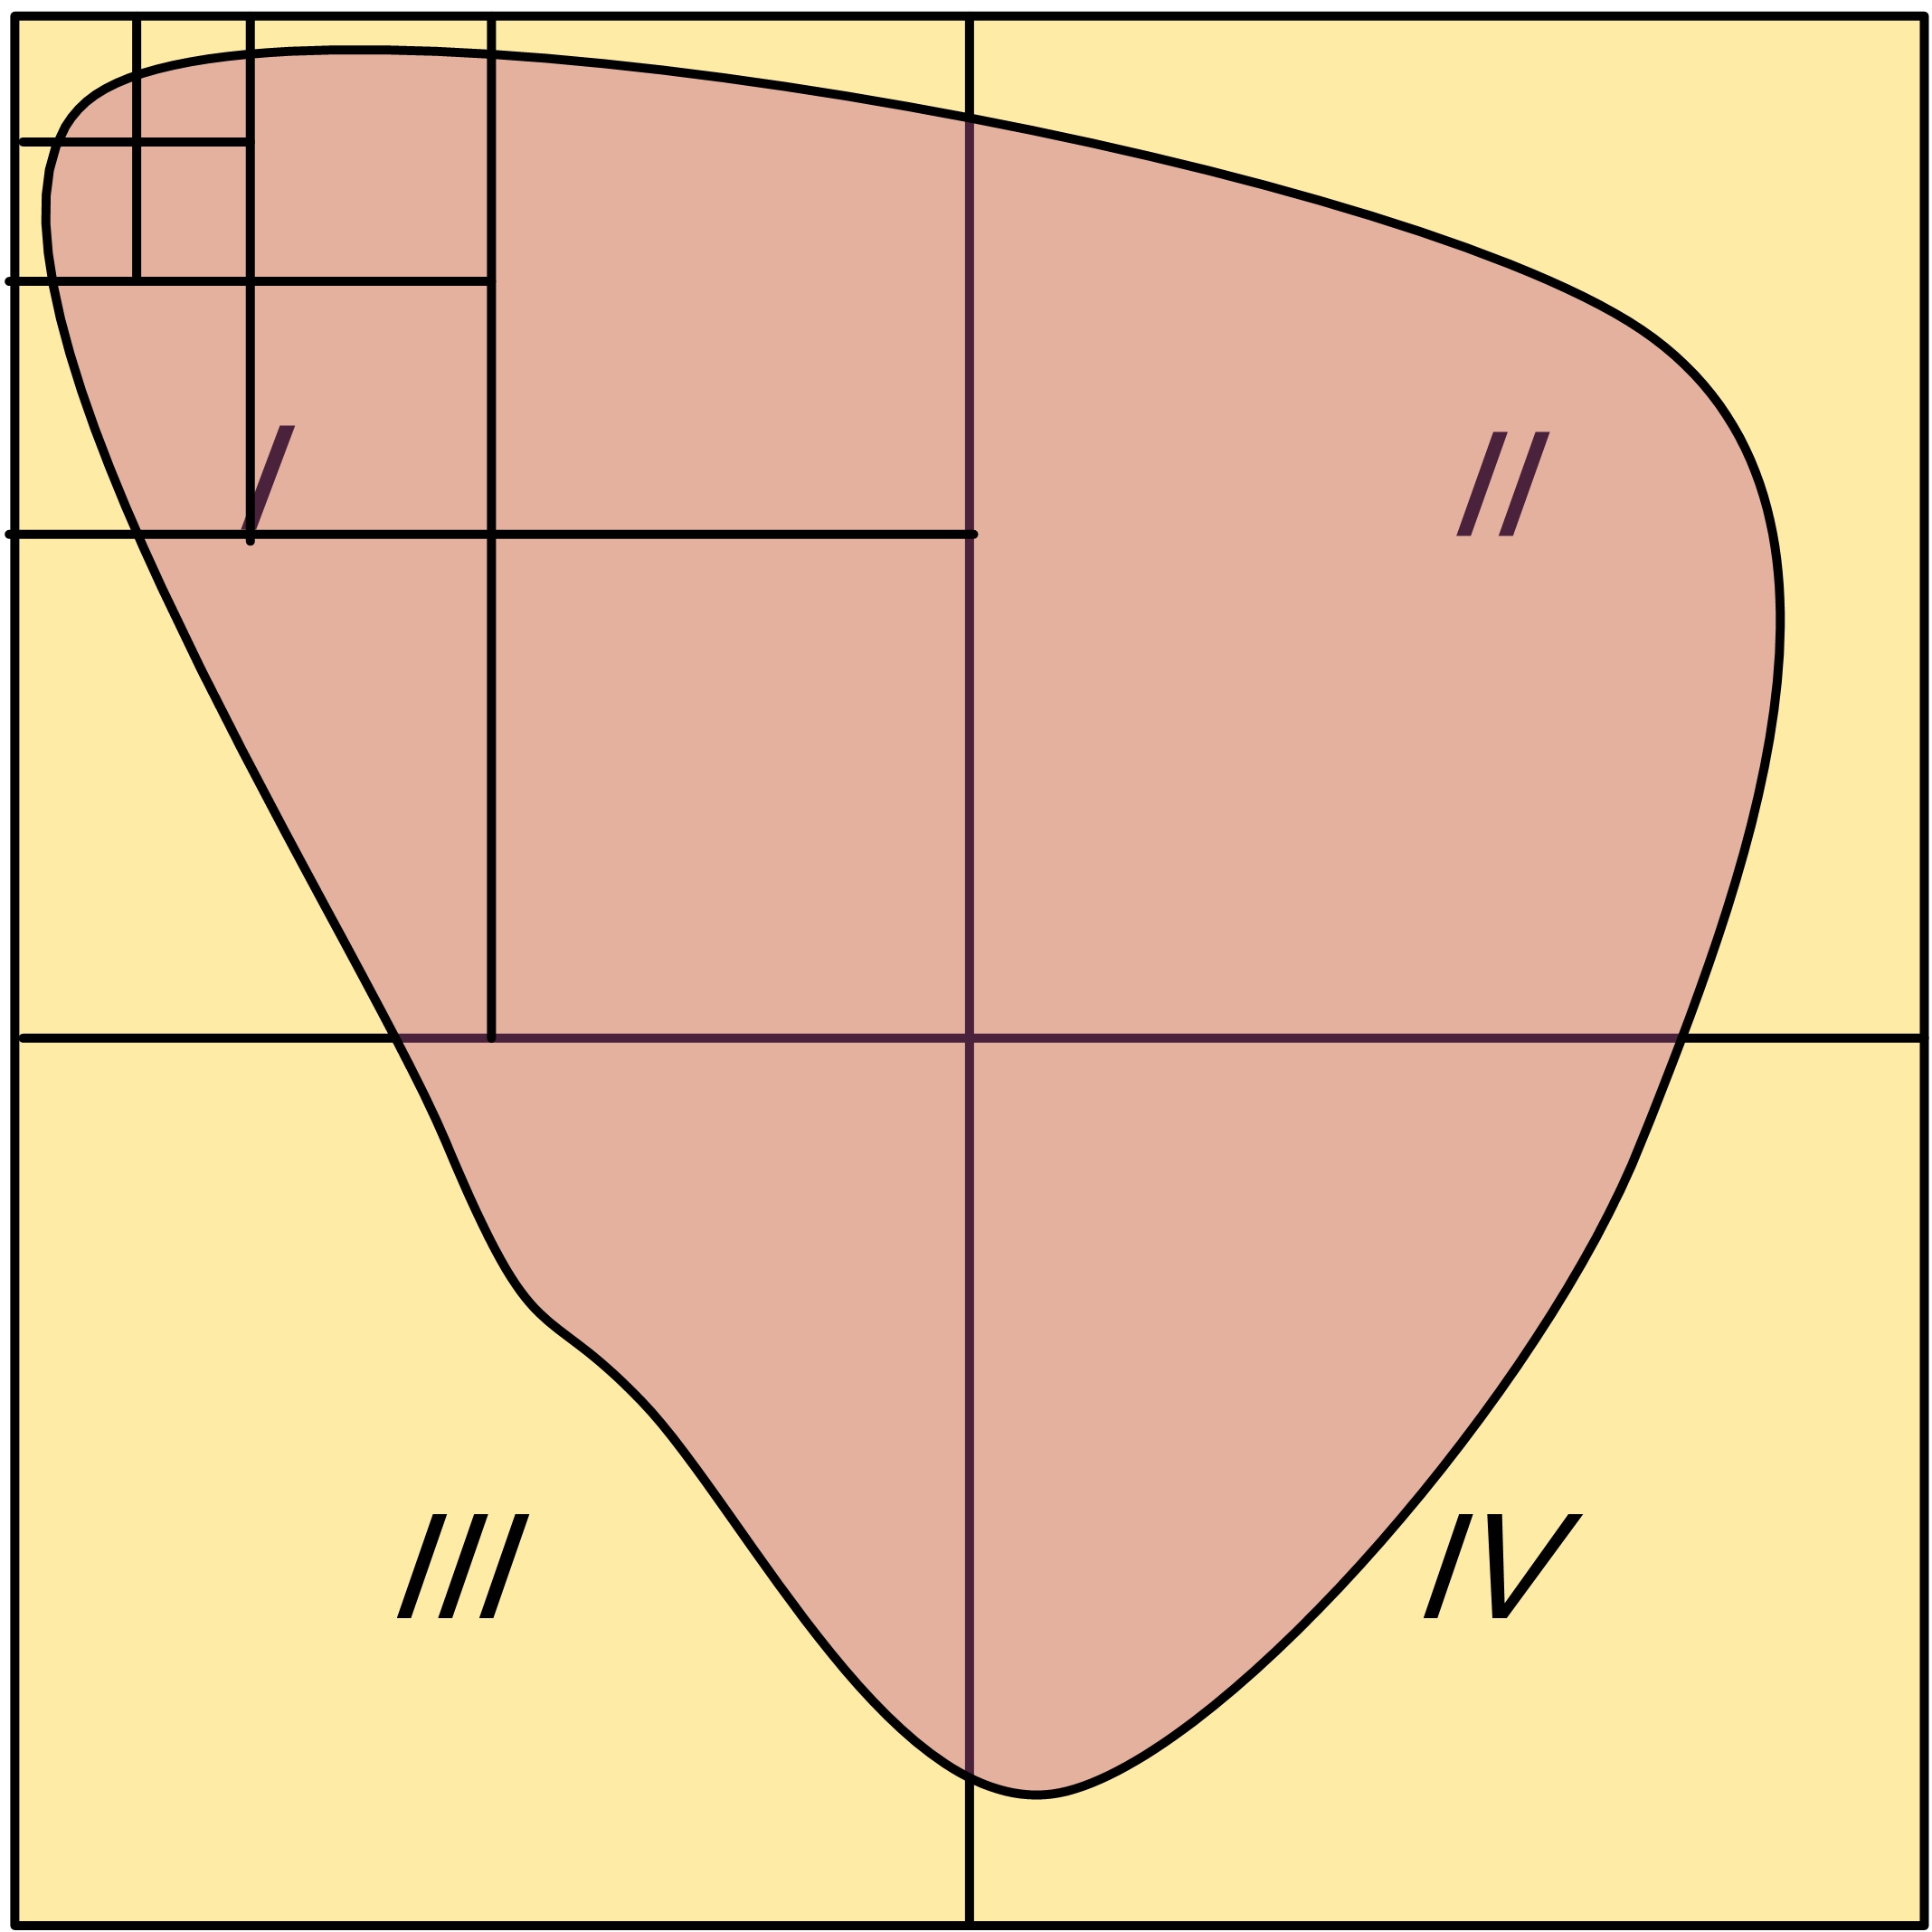
\includegraphics[width=0.2\linewidth]{Untitled}
	\caption{}
	\label{fig:untitled}
\end{figure}

如图(1.1),我们将其该矩形四等分,则存在一些区域无法被有限个开覆盖覆盖,不失一般性,不妨假设是在Ⅰ区在一区中,我们将其四等分,同样能找到不能被有限个开覆盖覆盖的区域,类似的,我们多次将其四等分,构成了一系列的非空的区间套,这些区间不能被有限个开覆盖覆盖,由区间套定理,我们可以找到一个唯一的$x\in E$,并且其不能被有限个开区间覆盖,但显然$B(x,\delta)$可覆盖住$x$,矛盾。于是原命题得证
\end{proof}
\begin{definition}
	$\text{设}E\subset \mathbb{R} ^n$,如果$E $的任一分解式$ E =A\cup B$满足$A\ne \oslash$,$B\ne\oslash$且$A\cap B= \oslash $,则可以得到下面两式
	\begin{equation*}
		A\cap B'\ne \oslash ,A'\cap B\ne \oslash 
	\end{equation*}
	中至少有一个成立,则称 $E$ 为$ \mathbb{R} ^n$ 中的连通集,或者说$ E$ 是连
	通的
\end{definition}
\begin{definition}
	在$ \mathbb{R} ^n$ 中,连通的开集称为区域,区域的闭包称为闭
	区域
\end{definition}
\begin{theorem}
	开集$E\subset  \mathbb{R} ^n$为连通集的充要条件是$E $不能分解为
	两个不相交的非空开集的并
\end{theorem}
\begin{proof}
	$\Rightarrow$
	
	假设其能分解为两个不相交的非空开集的并,
	即
	\begin{equation*}
		E=A\cup B; A,B\ne \oslash ;A\cap B=\oslash 
	\end{equation*}
	
	于是
	\begin{equation*}
		\forall x\in A,\exists r,\text{使得}B\left( x,r \right) \subset A
	\end{equation*}
	
	故
	\begin{equation*}
		B\left( x,r \right)\cap B'=\oslash
	\end{equation*}
	
	同样的,也可证明
	\begin{equation*}
		\forall y \in B \exists d, B\left( y,d \right)\cap A'=\oslash
	\end{equation*}
	
	与连通集矛盾。
	
	$\Leftarrow$
	
	设其不连通,则
	
	\begin{equation*}
		E=A\cup B;A,B\ne \oslash ;A\cap B=\oslash ;A\cap B'=\oslash,B\cap A'=\oslash
	\end{equation*}
	
	下证$A,B$为开集,由$A\cap B'=\oslash$
	\begin{equation*}
		\forall x \in A ,\exists r \text{使得}B(x,r)\cap B=\oslash
	\end{equation*}
	
	又因为
	\begin{equation*}
		x\notin B
	\end{equation*}
	
	于是
	\begin{equation*}
		\exists r>0,B(x,r)\subset A
	\end{equation*}
	
	因此$A$为开,同理$B$为开,与命题矛盾
\end{proof}
\section{2023/9/11}
\begin{theorem}
	在  $\mathbb{R}$上集合 $E$ 连通的充要条件是$ E$ 为区间。
\end{theorem}
\begin{proof}
	
	我们需要用到下面的引理
	\begin{equation*}
		E\text{为区间的充要条件是}\forall a,b\in E,\left[ a,b \right] \subset E
	\end{equation*}
	
	$\Rightarrow$

	我们采取反证法,即
	\begin{equation*}
		\exists c,d \in E,\text{有}[c,d]\nsubset E
	\end{equation*}
	
	立即推出
	\begin{equation*}
		\exists x_{0} \in [c,d] ,x_{0}\notin E 
	\end{equation*}
	
	令$\begin{cases}
		A=\left\{ x\in E|x<x_0 \right\}\\
		B=\left\{ x\in E|x>x_0 \right\}\\
	\end{cases}$,
	由于$E$连通,则
	\begin{equation*}
		E=A\cup B;A,B\ne \oslash ;A\cap B=\oslash ;A\cap B'\ne\oslash\text{或}B\cap A'\ne\oslash
	\end{equation*}
	
	$\forall y \in A' $,我们有
	\begin{equation*}
		\exists \left\{ y_n \right\} \subset A,y_n\ne y,\lim_{n\rightarrow \infty} y_n=y
	\end{equation*}
	
	于是有
	\begin{equation*}
		y\le x_{0}
	\end{equation*}
	
	故
	\begin{equation*}
		y\notin B\Rightarrow B\cap A'=\oslash
	\end{equation*}
	
	矛盾
	
	$\Leftarrow$
	
	令\begin{equation*}
		E=A\cup B;A,B\ne \oslash ;A\cap B=\oslash 
	\end{equation*}
	
	只需证明
	\begin{equation*}
		A\cap B'\ne\oslash\text{或}B\cap A'\ne\oslash
	\end{equation*}
	
	即可
	
	我们如下构造区间套
	
	取$a_{1}\in A,b_{1}\in B$,令$c_{1}=\frac{a_{1}+b_{1}}{2}$,如果$c_{1}\in A$,令$a_{2}=c_{1},b_{2}=b_{1} $,如果$c_{1}\in B$,令$b_{2}=c_{1},a_{2}=a_{1} $
	
	令$c_{2}=\frac{a_{2}+b_{2}}{2}$,如果$c_{2}\in A$,令$a_{3}=c_{2},b_{3}=b_{2} $,如果$c_{2}\in B$,令$b_{3}=c_{2},a_{3}=a_{2} $
	
	$\cdots$
	
	多次循环,我们可得到一个区间套$[a_{n},b_{n}]$,且其直径趋向于零,由区间套定理
	
	\begin{equation*}
		\exists \text{唯一的}\xi \in [a_{n},b_{n}],\lim_{n\rightarrow \infty} a_n=\lim_{n\rightarrow \infty} b_n=\xi 
	\end{equation*}
	
	如果$\xi \in A$,则$\xi \in B'$,即$A\cap B'\ne\oslash$,同理可证$B\cap A'\ne\oslash$
	
	下证引理
	
	\begin{equation*}
		E\text{为区间的充要条件是}\forall a,b\in E,\left[ a,b \right] \subset E
	\end{equation*}
	
	\begin{proof}
		$\Rightarrow$
		
		显然
		
		$\Leftarrow$
		
		记$\mathrm{inf}E=-\infty \text{或}a,\mathrm{sup}E=+\infty \text{或}b$
		
		我们要证明$E=[a,+\infty)$(不失一般性)
		
		显然,我们有
		\begin{equation*}
			E\subset[a,+\infty)
		\end{equation*}
		
		下证
		\begin{equation*}
			[a,+\infty)\subset E
		\end{equation*}
		
		$\forall x \in [a,+\infty)$,我们只需证明$x\in E$即可
		
		1.若$a \in E$,则对于上述的$x$,我们有
		$a\le x$恒成立,由于$\mathrm{sup}E=+\infty$,于是$\exists N>0\in E,a<N$,于是$x\in [a,N]\subset E$,结论成立。
		
		2.若$a \notin E$,则此时结论不成立
		
		综上$E$为区间
	\end{proof}
\end{proof}
\begin{definition}
	设$E\subset  \mathbb{R} ^n$,如果对任意两点$ p, q \in E$,都有一条连
	续曲线 $l \subset E $将$ p, q$ 连接起来,则称点集$ E$ 是道路连通的
\end{definition}
\begin{theorem}
	道路连通集一定是连通集
\end{theorem}
\begin{proof}
	
	不妨设$E$道路连通,下证其为连通集
	
	令\begin{equation*}
		E=A\cup B;A,B\ne \oslash ;A\cap B=\oslash 
	\end{equation*}
	
	只需证明
	\begin{equation*}
		A\cap B'\ne\oslash\text{或}B\cap A'\ne\oslash
	\end{equation*}
	
	即可
	
	取$p\in A,q\in B$,由于$E$道路连通,则存在一个向量函数$\Phi \left( t \right) ,t\in \left[ 0,1 \right] $,使得
	\begin{equation*}
		\Phi \left( 0 \right)=p,\Phi \left( 1 \right)=q
	\end{equation*}
	令$\begin{cases}
		S=\left\{ t\in \left[ 0,1 \right] |\Phi \left( t \right) \in A \right\}\\
		T=\left\{ t\in \left[ 0,1 \right] |\Phi \left( t \right) \in B \right\}\\
	\end{cases}$
	
	显然有
	\begin{equation*}
		S\cup T=\left[ 0,1 \right] ,S\ne \oslash ,T\ne \oslash ,S\cap T=\oslash 
	\end{equation*}
	(这里我们采用了一种部分代替整体的手法,可以积累一下)
	
	由于[0,1]为连通的,则有
	\begin{equation*}
			S\cap T'\ne\oslash\text{或}T\cap S'\ne\oslash
	\end{equation*}
	
	不妨设$S\cap T'\ne \oslash \text{,取}x\in S\cap T',\text{则有}\left\{ x_n \right\} \subset T,\text{使得}\lim_{n\rightarrow \infty} x_n=x\left( x_n\ne x \right)$ 
	
	于是有
	\begin{equation*}
		\Phi \left( x \right)\in A,\Phi \left( x_{n} \right)\in B
	\end{equation*}
	
	由于$\Phi \left( t \right)$连续,则
	\begin{equation*}
		|\Phi\left( x_{n} \right)-\Phi \left( x \right)|<\varepsilon
	\end{equation*}
	于是$\Phi \left( x \right)\in B'$,结论得证
\end{proof}
\begin{example}
	连通集未必是道路连通的,例如,设集合
	\begin{equation*}
		E=\left\{ \left( x,y \right) \in \mathbb{R} ^2|y=\sin \frac{1}{x},0<x\le \frac{2}{\pi} \right\}
	\end{equation*}
	该曲线被称为“拓扑学家的正弦曲线”,则可以证明:$\bar{E}$ 是连通
	的,但不是道路连通的
\end{example}
\begin{proof}
	
	反证:
	
	设$\bar{E}$不连通,则
	
	\begin{equation*}
		\bar{E}=A\cup B;A,B\ne \oslash ;A\cap B=\oslash ;A\cap B'=\oslash,B\cap A'=\oslash
	\end{equation*}
	
	令$A_{1}=A\cap E,B_{1}=B\cap E$
	
	则有$E=A_{1}\cup B_{1}$
	
	显然有
	\begin{equation*}
		A_{1}\cap B_{1}=\oslash ;A_{1}\cap B'_{1}=\oslash,B_{1}\cap A'_{1}=\oslash
	\end{equation*}
	
	现我们只需证明$A_{1},B_{1}$非空即可
	
	若$A_{1}=\oslash$,由$A_{1}=A\cap E,B_{1}=B\cap E$,则$A\subset E'$,此时$E=B_{1}\subset B$
	
	$\forall x\in A$,由于$A\subset E'$,$E=B_{1}\subset B$,我们有
	\begin{equation*}
		\exists \left\{ x_n \right\} \subset B,\underset{n\rightarrow \infty}{\lim}x_n=x\left( x_n\ne x \right)
	\end{equation*}
	
	于是$x\in B'$,与题目$A_{1}\cap B_{1}'=\oslash$矛盾,于是$A_{1}$非空,同理$B_{1}$非空
	
	于是对$E$有
	\begin{equation*}
			E=A_{1}\cup B_{1};A_{1},B_{1}\ne \oslash ;A_{1}\cap B_{1}=\oslash ;A_{1}\cap B_{1}'=\oslash,B_{1}\cap A_{1}'=\oslash
	\end{equation*}
	
	于是$E$非连通集,显然矛盾
	
	因此$\bar{E}$连通
	
	不妨设其道路连通,则存在一个向量函数$\Phi \left( t \right) ,t\in \left[ 0,1 \right] $,使得
	\begin{equation*}
		\Phi \left( 0 \right)=(0,0),\Phi \left( 1\right)=(\frac{2}{\pi},1)
	\end{equation*}
	
	由介值定理$\text{存在}0<t_1<1$,使得
	\begin{equation*}
		\Phi \left( t_1 \right) =\left( \frac{1}{\frac{\pi}{2}+\pi},\sin \left( \frac{\pi}{2}+\pi \right) \right)
	\end{equation*}
	
	介值定理$\text{存在}0<t_2<t_{1}<1$,使得
	\begin{equation*}
		\Phi \left( t_2 \right) =\left( \frac{1}{\frac{\pi}{2}+2\pi},\sin \left( \frac{\pi}{2}+2\pi \right) \right)
	\end{equation*}
	
	$\cdots$
	
	多次构造,我们得到一个单调递减有下界的数列$\left\{ t_n \right\} $,显然其极限存在,但此时$\Phi \left( t_n \right)=\left( \frac{1}{\frac{\pi}{2}+n\pi},\sin \left( \frac{\pi}{2}+n\pi \right) \right)$极限却不存在,这与道路连通矛盾,于是不道路连通
\end{proof}
\begin{example}
	在  $\mathbb{R} ^n$中,开球是区域
\end{example}
\section{习题部分}
\begin{exercise}
	试证明在一个度量空间中,半径为 7 的球不可能成为半径为
	3 的球的真子集
\end{exercise}
\begin{proof}
	直接证明不好证明,我们反着来
	
	$\left\| x-a \right\| <7\Rrightarrow \left\| x-b \right\| <3$
	
	但事实上,若$\left\| a-b \right\| <4$,对$\left\| x-b \right\|<3$ 
	
	则$\left\| x-a \right\| =\left\| x-a+a-b \right\| <\left\| a-b \right\| +\left\| x-b \right\| <4+3=7$,与条件半径7的球为半径3的球的真子集矛盾
\end{proof}
\begin{exercise}
	证明:欧氏空间的基本列必是有界的
\end{exercise}
\begin{proof}
	设$x_{n}$为基本列,则$\forall \varepsilon >0 \exists N,i,j$,当$i,j>N$时,有
	\begin{equation*}
		\left\| x_i-x_j \right\| <\varepsilon 
	\end{equation*}

	固定住$j$,我们有
	\begin{equation*}
		\left\| x_i \right\| =\left\| x_i-x_j+x_j \right\| <\left\| x_i-x_j \right\| +\left\| x_j \right\| =\varepsilon +\left\| x_j \right\| 
	\end{equation*}
	得证
\end{proof}
\begin{exercise}
	针对以下各题中指定的集合 $A$,求出 $A\degree$,$\bar{A}$和 $\partial 	A$(直接写
	结论即可)
	
	1.$\text{在}\mathbb{R} \text{中,}A=\left\{ 1\text{,}\frac{1}{2}\text{,}\frac{1}{3}\text{,}\cdots \right\} $
	
	2.$A\text{为}\mathbb{R} ^n\text{中的有限点集}$
	
	3.$\text{在}\mathbb{R} ^2\text{中,设}A=\left\{ \left( x,y \right) |x,y\in \mathbb{Q} \right\} $
\end{exercise}
\begin{solution}
	
	1.$A\degree=\oslash ;\bar{A}=A \cup \left\{ 0 \right\} ;\partial A=A\cup \left\{ 0 \right\} $
	
	2.$A\degree=\oslash ;\bar{A}=A ;\partial A=A$
	
	3.$A\degree=\oslash ;\bar{A}=\mathbb{R} ^2;\partial A=\mathbb{R} ^2$
\end{solution}
\begin{exercise}
	证明$p \in \bar{A}$的充要条件是对任意$r>0$,有$B_{r}(p)\cap A \ne \oslash$
\end{exercise}
\begin{proof}
	
	$\Rightarrow$
	
	若$p\in A$,结论显然成立
	
	若$p\in A'$,则$\forall r_{1}>0$,使得$\check{B}(p,r_{1})\cap A\ne\oslash$
	
	必要性得证
	
	$\Leftarrow$ 
	
	我们取$\left\{ p_n \right\} \subset B(p,r)\cap A\ne\oslash$使得$\underset{n\rightarrow \infty}{\lim}p_n=p$,则$\forall r_{1}>0$,使得$\check{B}(p,r_{1})\cap A\ne\oslash$
	
	故$p\in A'\subset \bar{A}$
	
	充分性得证
\end{proof}
\begin{exercise}
	设$E\subset \mathbb{R} ^n$,求证$\partial E$为闭集
\end{exercise}
\begin{proof}
	
	这里我们要用到定理$(1.1)$,$\text{取}\left\{ x_n \right\} \subset \partial E,\text{并且}\underset{n\rightarrow +\infty}{\lim}x_n=x$,下证$x\in \partial E$
	
	由于$\underset{n\rightarrow +\infty}{\lim}x_n=x$,$\forall \varepsilon >0 ,\exists N,\text{当}n>N$,有
	\begin{equation*}
		\left\| x_n-x \right\| <\varepsilon 
	\end{equation*}
	
	类似于定理$(1.3)$的取法,我们也可构造一个$\left\{ m_n \right\}\subset E $使得$\underset{n\rightarrow +\infty}{\lim}m_n=x_{n}$
	
	于是乎,对于上述$\varepsilon,\exists N,n>N$时,有
	\begin{equation*}
		\left\| m_n-x \right\| =\left\| m_n-x_n+x_n-x \right\| <\left\| m_n-x_n \right\| +\left\| x_n-x \right\| <2\varepsilon 
	\end{equation*}
	
	于是$\underset{n\rightarrow +\infty}{\lim}m_n=x$,则
	$\forall r>0$,使得$B(x,r)\cap E\ne\oslash$
	
	同样的,我们也可证明$\forall r>0$,使得$B(x,r)\cap E^{c}\ne\oslash$
	
	即$x\in \partial E$
\end{proof}
\begin{exercise}
	$E$ 为闭集的充要条件是 $\partial E \subset E$
\end{exercise}
\begin{proof}
	$\Rightarrow$
	
	现我们需证明$\forall x \in \partial E,x\in E$,$\text{不妨假设}x\notin E$,
	
	$E$为闭集,则$E^{c}$为开,即$\exists r>0$,使得$B(x,r)\cap E=\oslash$
	
	这与$\forall x \in \partial E$矛盾
	
	$\Leftarrow$
	
	不妨假设$E$为开,即$\exists r>0$,使得$B(x,r)\cap E^{c}= \oslash$
	
	任取$x \in \partial E$,则$\forall r>0,B(x,r)\cap E^{c}\ne \oslash$,又$\partial E \subset E$,则$x\in E$,与假设矛盾
\end{proof}
\begin{exercise}
	$\text{设}F_1,F_2,\cdots ,F_n\text{为}\mathbb{R} ^n\text{的非空闭集}$,满足$F_{k+1}\subset F_k(k\le 1)$,问是否一定有$\bigcap_{k=1}^{\infty}{F_k}\ne \oslash $,若改为非空
	紧集又如何?
\end{exercise}
\begin{solution}
	
	若不能保证其为有界闭集,则结果不一定成立。但改为非空紧集则一定有。理由如下。
	
	$\text{若}\bigcap_k{F_k}=\oslash $
	
	$\text{则取补集,有}\bigcup_k{F_{k}^{c}}=\mathbb{R} ^n$
	
	$\text{于是}\left\{ F_{k}^{c},k\ge 1 \right\} \text{构成了紧集}F_1\text{的开覆盖}$
	
	$\text{根据紧集的性质,可以从中取出有限覆盖}F_{k_1}^{c},F_{k_2}^{c},\cdots ,F_{k_n}^{c}$
	
	$\text{由于其具有包含的关系,不妨记}F_{k_n}^{c}\text{为最大的有限覆盖}$

	
	$\text{即}F_1\subset F_{k_n}^{c}\Rrightarrow F_1\cap F_{k_n}^{}=\oslash ,\text{这与子集相交不为空矛盾}$
\end{solution}
\begin{exercise}
	设$E\subset \mathbb{R} ^n$为一有界闭集,$\left\{ G_{\alpha} \right\} \text{为}E\text{的一个开覆盖}$,$\text{证明:必存在}\sigma >0\text{(通常称该数为开覆盖}G_{\alpha}\text{的}Lebesgue\text{数)}$,使得只要集合$F\subset\mathbb{R} ^n $满足条件
	\begin{equation*}
		F\cap E\ne \oslash,\mathrm{diam}F<\sigma 
	\end{equation*}
	就能断言$F$能被$\left\{ G_{\alpha} \right\} $的某个开集所覆盖
\end{exercise}
\begin{proof}
	反证法:
	
$\forall	\sigma >0$,集合$F\subset\mathbb{R} ^n $满足条件
	\begin{equation*}
		F\cap E\ne \oslash,\mathrm{diam}F<\sigma 
	\end{equation*}
	
	$F$都不能能被$\left\{ G_{\alpha} \right\} $的某个开集所覆盖
	
	翻译成数学语言就是
	\begin{equation*}
		\forall \sigma >0,\exists F\cap E\ne\oslash,|F|<\sigma ,\forall i\in \alpha ,F   \nsubset G_i
	\end{equation*}
	
	可以推出
	\begin{equation*}
		\forall n\in N^*\,\,,\exists F\cap E\ne\oslash,|F|<\frac{1}{n},\forall i\in \alpha ,F_n\nsubset G_i
	\end{equation*}
	
	此时我们构造一个数列$\left\{ x_{n} \right\} $,使得
	\begin{equation*}
		 x_{n} \in F\cap E\ne\oslash
	\end{equation*}
	
	由聚点定理,可以从这数列中选取一个子列$\left\{ x_{n_{k}} \right\} $,使得其极限为$\xi \in E$
	
	现在取充分小的$\varepsilon$,使得
	\begin{equation*}
		\exists i\in \alpha ,B(\xi,\varepsilon)\subset G_{i}
	\end{equation*}
	
	对于上述的$\varepsilon$,由数列极限的性质$\exists N_{1}>0,n>N_{1}$,使得
	\begin{equation*}
	|x_n-\xi |<\frac{\varepsilon }{2}
	\end{equation*}
	
	同样存在$N_{2}>0,n>N_{2}$有
	\begin{equation*}
		|F_{n}|<\frac{\varepsilon}{2}
	\end{equation*}
	
	取$N=\max \left\{ N_1,N_2 \right\} ,n>N$有
	\begin{equation*}
		\forall x \in F_{n},|x-\xi |=|x-x_{n_k}+x_{n_k}-\xi |<|x-x_{n_k}|+|x_{n_k}-\xi |<\varepsilon 
	\end{equation*}
	
	这表明
	\begin{equation*}
		\exists N,n>N,\exists i\in \alpha ,\text{使得}F_n\subset   B(\xi,\varepsilon)\subset G_{i}
	\end{equation*}
	
	这与题设矛盾,于是原命题得证
\end{proof}
\begin{exercise}
	利用上题证明:设$E\subset \mathbb{R} ^n$为一有界闭集,$\left\{ G_{\alpha} \right\} \text{为}E\text{的一个开覆盖}$,则必能从$\left\{ G_{\alpha} \right\}$中选出有限个开集,它们仍能覆
	盖 $E$
\end{exercise}
\begin{proof}
	
	不妨假设有限个开集不能覆盖$E$,从$\left\{ G_{\alpha} \right\}$选取子集
	\begin{equation*}
		G_{n_1},G_{n_2},\cdots ,G_{n_k}
	\end{equation*}
	
	构成一个新的集合$\left\{ G_{n_{k}} \right\}$
	
	由题,则其不能覆盖$E$,即
	\begin{equation*}
		\exists x_{1} \in E,\text{但}x_{1}\notin \left\{ G_{n_{k}} \right\}
	\end{equation*}
	
	于是存在充分小的$\sigma$,使得$B(x,\frac{\sigma}{2})\subset E$
	
	由上题的结论,则
	\begin{equation*}
		\exists k_{1}\in \alpha,\text{使得}B(x_{1},\frac{\sigma}{2})\subset G_{k_{1}}
	\end{equation*}
	
	于是$\left\{ G_{n_{k}},G_{k_{1}} \right\}$构成一个新的子覆盖
	
	多次重复上述过程,则有一个新的子覆盖
	\begin{equation*}
		\left\{ G_{n_k},G_{k_1},G_{k_2},\cdots ,G_{k_n} \right\} 
	\end{equation*}
	
	满足
	\begin{equation*}
		\exists x_{n_{k}+k_{n}+1},\text{满足},x_{n_{k}+k_{n}+1}\in E,x_{n_{k}+k_{n}+1}\notin G_{n_1}\cup G_{n_2}\cup \cdots \cup G_{k_n}
	\end{equation*}
	
	由于$E$为有界闭集,则存在一个子序列		$\left\{ x_{n_{k}} \right\} ,\text{使得其极限为}\xi \in E$,对于充分大的$k$,有
	\begin{equation*}
		\left\| x_{n_k}-\xi \right\| <\sigma 
	\end{equation*}
	
	此时有
	\begin{equation*}
		\xi\in B(x_{n_{k}},\frac{\sigma}{2})\subset G_{n_{k}}
	\end{equation*}

	事实上,当$l>k$时,所有的$x_{n_{k}}$均发散至$B(x_{n_{k}},\frac{\sigma}{2})$的外面,与收敛矛盾。故选取$x_{n}$和$G_{n}$的过程应该在有限次终止
\end{proof}
\begin{exercise}
	证明:区域必是道路连通的
\end{exercise}
\begin{proof}
	反证,设区域两点内$a,b$没有道路联通,则定义
	$\begin{cases}
		A_1=\left\{ x\in X|\text{存在道路联通}x\text{和}a \right\}\\
		A_2=\left\{ x\in X|\text{不存在道路联通}x\text{和}a \right\}\\
	\end{cases}$
	
	显然$\left\{ \begin{array}{c}
		A_1,A_2\ne \oslash\\
		A_1\cap A_2=\oslash\\
		A_1\cup A_2=X\\
	\end{array} \right. $
	
	由于$X$为区域,$\forall x \in A_{1},\exists \delta>0$,使得$B(x,\delta)\subset X$,在这个邻域中的点恒与$x$能联通,于是$B(x,\delta)\subset A_{1}$则$A_{1}$为开集。同理可证明$A_{2}$为开集,于是$X$可分解为两个不相交开集的并,和为不连通矛盾。
\end{proof}
\begin{exercise}
	设$A \subset \mathbb{R} ^n$,如果$A$既为开集又为闭集,则$A=\oslash$或$A=\mathbb{R} ^n$
\end{exercise}
\begin{proof}
	设$E \subset \mathbb{R} ^n$,且$E\ne\oslash$,$E\ne\mathbb{R} ^n$
	
	由$E$既为开集又为闭集,则$E^{c}$既是开集又是闭集,作为两个不交的非空闭集,显然没有公共的边界点,与二者互为补集矛盾
\end{proof}
\chapter{多元函数的极限与连续}
\section{2023/9/12}
\begin{definition}
	设$E\subset \mathbb{R} ^n$,$f$ 是一个规律,如果对于 $E $中的任一点
	$x = (x_{1}, x_{2}, \cdots, x_{n})$,通过规律 $f$,在 $R $中都有唯一一个实数 $u$
	和此 $x$ 对应,就称$ f$ 为定义在 $E$ 上的一个 $n$ 元函数,
	$	x_{1}, x_{2}, \cdots , x_{n}$ 称为函数 $f $的 $n$ 个独立变量,$f$ 在 $(x_{1}, x_{2}, \cdots , x_{n})$
	的值为 $u$,记为 $u = f(x_{1}, x_{2}, \cdots , x_{n})$,通常采用如下符号记这个
	函数:
	\begin{equation*}
		\begin{split}
			f\text{:}E\rightarrow \mathbb{R} 
			\\
			\left( x_1,x_2,\cdots ,x_n \right) \longmapsto u=f(x_1,x_2,\cdots ,x_n)
		\end{split}
	\end{equation*}
	并称 $E$ 为 $f$ 的定义域。
\end{definition}
\begin{remark}
	
	1. 直流电路中,$I =\frac{U}{R}$确定了 $I$ 为 $U, R$ 的二元函数;
	
	2. 理想气体状态方程 $pV = RT$($R$ 为常数)根据问题的不同
	可以确定气体的体积、压力和温度中的一个为另外两个的二
	元函数。
\end{remark}
\begin{example}
	求函数$f\left( x,y \right) =\frac{\mathrm{arc}\sin \left( 3-x^2-y^2 \right)}{\sqrt{x-y^2}}$的定义域
\end{example}
\begin{solution}
	
	由题,有
	\begin{equation*}
		-1\le 3-x^2-y^2\le 1;x-y^2>0
	\end{equation*}
	
	解得
	\begin{equation*}
		2\le x^2-y^2\le 4;x>y^2
	\end{equation*}
	
	于是
	\begin{equation*}
		\left\{ \left( x,y \right) |2\le x^2-y^2\le 4;x>y^2 \right\} 
	\end{equation*}
\end{solution}
\begin{definition}
	设二元函数 $f(x, y) $的定义域为 $D$,对于任意取定的$ P(x, y) \in D$,
	对应的函数值为 $z = f(x, y)$,这样,以 $x $为横坐标、$y$ 为纵坐标、
	$	z$ 为竖坐标在空间就确定一点 $M(x, y, z)$,当 $(x, y)$ 取遍 $D$ 上一切
	点时,得一个空间点集 $\left\{ (x,y,z)|z=f(x,y),(x,y)\in D \right\}$,这个点
	集称为二元函数的图形。
\end{definition}
如下图所示,其为一个二元函数的图形
\begin{figure}[H]
	\centering
	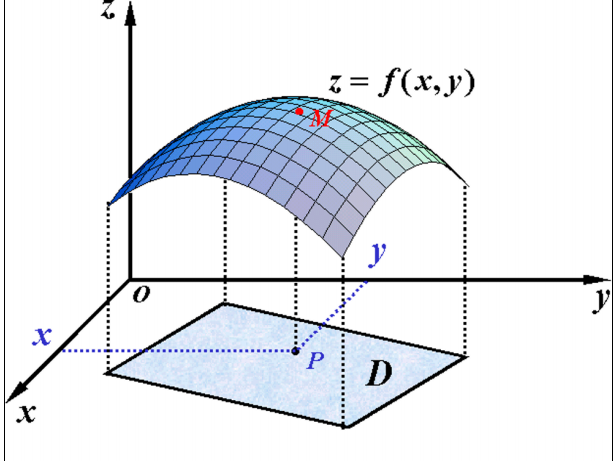
\includegraphics[width=0.2\linewidth]{screenshot001}
	\caption{}
	\label{fig:screenshot001}
\end{figure}

\begin{definition}
	$\text{设}D\subset \mathbb{R} ^n,f:D\rightarrow \mathbb{R} ,a\in \mathbb{R} ^n$为
\end{{definition}
\end{document}